%%%%%%%% ICML 2018 EXAMPLE LATEX SUBMISSION FILE %%%%%%%%%%%%%%%%%

\documentclass{article}

% Recommended, but optional, packages for figures and better typesetting:
\usepackage{microtype}
\usepackage{graphicx}
\usepackage{caption}
\usepackage{subcaption}
\usepackage{booktabs} % for professional tables

% hyperref makes hyperlinks in the resulting PDF.
% If your build breaks (sometimes temporarily if a hyperlink spans a page)
% please comment out the following usepackage line and replace
% \usepackage{icml2018} with \usepackage[nohyperref]{icml2018} above.
\usepackage{hyperref}

% Attempt to make hyperref and algorithmic work together better:
\newcommand{\theHalgorithm}{\arabic{algorithm}}

% Use the following line for the initial blind version submitted for review:
\usepackage{icml2018}
\usepackage{natbib}
\usepackage{amsmath}
\usepackage{amsthm}
\usepackage{amsfonts}
\usepackage{bbm}
\usepackage{bm}
\usepackage{amssymb}
\newtheorem{theorem}{Theorem}
\newtheorem{proposition}[theorem]{Proposition}
\newtheorem{definition}{Definition}
\makeatletter
\renewenvironment{proof}[1][\proofname]{\par
  \vspace{-\topsep}% remove the space after the theorem
  \pushQED{\qed}%
  \normalfont
  \topsep0pt \partopsep0pt % no space before
  \trivlist
  \item[\hskip\labelsep
        \itshape
    #1\@addpunct{.}]\ignorespaces
}{%
  \popQED\endtrivlist\@endpefalse
  \addvspace{0pt plus 0pt} % some space after
}
\makeatother

% Supplementary File
\usepackage{xr-hyper}
\externaldocument[Su-]{Supplementary}

% If accepted, instead use the following line for the camera-ready submission:
%\usepackage[accepted]{icml2018}

% The \icmltitle you define below is probably too long as a header.
% Therefore, a short form for the running title is supplied here:
\icmltitlerunning{Incentivizing High Quality Crowdsourcing Information using Bayesian Inference and Reinforcement Learning}

\begin{document}

\twocolumn[
\icmltitle{Incentivizing High Quality Crowdsourcing Information using\\Bayesian Inference and Reinforcement Learning}

% It is OKAY to include author information, even for blind
% submissions: the style file will automatically remove it for you
% unless you've provided the [accepted] option to the icml2018
% package.

% List of affiliations: The first argument should be a (short)
% identifier you will use later to specify author affiliations
% Academic affiliations should list Department, University, City, Region, Country
% Industry affiliations should list Company, City, Region, Country

% You can specify symbols, otherwise they are numbered in order.
% Ideally, you should not use this facility. Affiliations will be numbered
% in order of appearance and this is the preferred way.
\icmlsetsymbol{equal}{*}

\begin{icmlauthorlist}
\icmlauthor{Zehong Hu}{NTU}
\icmlauthor{Yang Liu}{Harvard}
\icmlauthor{Yitao Liang}{UCLA}
\icmlauthor{Jie Zhang}{NTU}
\end{icmlauthorlist}

%\icmlaffiliation{NTU}{Rolls-Royce Cooperate Lab@NTU, School of Computer Science and Engineering, Nanyang Technological University, Singapore}
%\icmlaffiliation{goo}{Googol ShallowMind, New London, Michigan, USA}
%\icmlaffiliation{ed}{School of Computation, University of Edenborrow, Edenborrow, United Kingdom}

%\icmlcorrespondingauthor{Cieua Vvvvv}{c.vvvvv@googol.com}
%\icmlcorrespondingauthor{Eee Pppp}{ep@eden.co.uk}

% You may provide any keywords that you
% find helpful for describing your paper; these are used to populate
% the "keywords" metadata in the PDF but will not be shown in the document
\icmlkeywords{Machine Learning, ICML}

\vskip 0.3in
]

% this must go after the closing bracket ] following \twocolumn[ ...

% This command actually creates the footnote in the first column
% listing the affiliations and the copyright notice.
% The command takes one argument, which is text to display at the start of the footnote.
% The \icmlEqualContribution command is standard text for equal contribution.
% Remove it (just {}) if you do not need this facility.

%\printAffiliationsAndNotice{}  % leave blank if no need to mention equal contribution
%\printAffiliationsAndNotice{} % otherwise use the standard text.

\begin{abstract}
This document provides a basic paper template and submission guidelines.
Abstracts must be a single paragraph, ideally between 4--6 sentences long.
Gross violations will trigger corrections at the camera-ready phase.
\end{abstract}

\section{Introduction}
\subsection{Motivation}
Peer prediction mechanisms have two fatal drawbacks:
\begin{itemize}
\item Existing peer prediction mechanisms only care about incentive compatibility (IC) which only poses requirements to the expected incentives to workers. They achieve IC via comparing the reports between the targeted and selected reference agents. In this way, they only use a tiny part of the information behind all collected labels. Besides, they never analyze the stochastic property of incentives and the variation of incentives among different types of agents.
\item Existing peer prediction mechanisms simplify workers' responses to the incentive mechanism by assuming that workers are all fully rational and only follow the utility-maximizing strategy. However, there is strong evidence showing that human workers are not always fully rational, and they may deviate from equilibrium strategies. Thus, these peer prediction mechanisms which is fancy in theory may yet fail in practice.
\end{itemize}

\subsection{Contribution}
We have two core contributions in this paper:
\begin{itemize}
\item We propose a novel one-shot peer prediction mechanism based on Bayesian inference. Since existing Bayesian inference algorithms (e.g. EM estimator and variational inference) for crowdsourcing are biased in principle, we derive the explicit posterior distribution of the true labels and employ Gibbs sampling for inference. The most challenging problem of our mechanism is to prove the incentive compatibility of our mechanism which has never been explored in the literature. Besides, we also empirically show the advantages of our mechanism on the stability and fairness of incentives over existing ones.
\item We design the first reinforcement peer prediction framework which sequentially interacts with workers. It dynamically adjusts the scaling level of our peer prediction mechanism to maximize the utility of the data requester. To avoid assuming a decision-making model for workers, we use the data-driven Gaussian process to represent the scaling level adjustment policy, and online updates our policy according to workers' responses. We theoretically prove the incentive compatibility of our framework and empirically show its advantages on improving the utility if the data requester over one-shot mechanisms.
\end{itemize}

\section{Related Work}

\section{Learning-Based Peer Prediction}
\subsection{Formulation and settings}
Suppose there is one data requester who assigns $M$ tasks with answer space $\left\{1,2\right\}$ to $N \geq 3$ candidate workers at each step $t=1,2\ldots T$.
We denote the tasks and workers by $\mathcal{T}^{t}=\{1,2,\ldots,M\}$ and $\mathcal{C}=\{1,2,\ldots,N\}$, respectively.
The label $L^{t}_{i}(j)$ generated by worker $i\in \mathcal{C}$ for task $j\in\mathcal{T}^{t}$ comes from a distribution that depends both on the ground-truth label $L^{t}(j)$ and worker $i$'s effort level $e^{t}_i$ and reporting strategy $r^{t}_i$.
Suppose there are two effort levels, High ($e^{t}_i=1$) and Low ($e^{t}_i=0$), that a worker can potentially choose from.
Meanwhile, worker $i$ can decide either to truthfully report his observation $r^{t}_i = 1$ or to revert the answer $r^{t}_i = 0$.
Note that worker $i$'s effort level and reporting strategy may be a mixed of the above pure actions.
Thus, we use $e^{t}_i\in[0,1]$ and $r^{t}_i\in[0,1]$ to denote worker $i$'s probability of exerting high efforts and being truthful, respectively.
Using the above notations, we can define worker $i$'s score (i.e. the probability of providing the correct label)  as
\begin{equation}
\begin{split}
&p^{t}_i=r^{t}_i e^{t}_i p_{i, H}+r^{t}_i (1-e^{t}_i) p_{i, L}+\\
&(1-r^{t}_i) e^{t}_i (1-p_{i, H})+(1-r^{t}_i) (1-e^{t}_i) (1-p_{i, L})
\end{split}
\end{equation}
where $p_{i, H}$ and $p_{i, L}$ denote the probability of observing the correct label when worker $i$ exerts high and low efforts, respectively.
Following the previous studies on peer prediction~\cite{dasgupta2013crowdsourced,liu2017sequential}, we assume that all workers share the same set of $p_{i, H}, p_{i, L}$, denoting by $p_H, p_L$, and $p_{H}>p_{L}\geq 0.5$.
Besides, we also assume these crowdsourcing tasks are homogeneous.

\subsection{One-Step Incentive Mechanism}
Now, we present our mechanism designed for inducing truthful reports and high efforts in one step:
\begin{definition}
\label{MechDef}
Denote worker $i$'s score estimated by using the Bayesian inference algorithm developed later in this section as $\tilde{p}^{t}_i$. Then, at step $t$, our mechanism computes worker $i$'s rewards for her reports on $M$ tasks as:
\begin{equation}
R^t(i)=M\cdot [a\cdot (\tilde{p}^{t}_i - 0.5)+b]
\end{equation}
where $a>0$ and $b\geq 0$ are the scaling level and the guaranteed base payment, respectively.
\end{definition}
There have been many inference algorithms developed in the literature of crowdsourcing~\cite{zheng2017truth}. Among them, the most popular one is the EM estimator~\cite{dawid1979maximum}. Another widely-adopted algorithm is the variational inference estimator~\cite{liu2012variational} which is similar to the EM estimator~\cite{tzikas2008variational}.
However, these estimators are irredeemably biased since the EM estimator may converge to the local optimum.
On the other hand, sampling-based Bayesian inference algorithms, for example Gibbs sampling, are computationally very expensive, even though they use the explicit posterior distribution and can avoid the inference bias.
Especially, workers' scores are continuous variables, which will significantly slow down the convergence speed.
Therefore, to the best of my knowledge, sampling-based Bayesian inference is never used for crowdsourcing where the number of workers and tasks is usually very large.
In this section, to reduce the inference bias and meanwhile avoid overly large computation costs, we firstly assume Dirichlet priors for those continuous variables in our system and derive a joint posterior distribution which only contains the discrete variables.
Then, we use Gibbs sampling to sample the obtained posterior distribution and estimate workers' scores based on those samples.

Specially, the joint distribution of the collected labels $\mathcal{L}=[L_i(j)]$ and true labels $\bm{L}=[L(1),\ldots, L(M)]$ satisfies\footnote{In this section, we only focus on developing the one-step mechanism and thus omit the superscript $t$ of all variables.}
\begin{equation}
\label{JointDist}
\begin{split}
    &P(\mathcal{L},\bm{L}| \bm{p}, \bm{\tau})=\\ &\qquad \prod_{j=1}^{M}\prod_{k=1}^{K}\left\{\tau_{k}\prod_{i=1}^{N}p_i^{\delta_{ijk}}(1-p_i)^{\delta_{ij(3-k)}} \right\}^{\xi_{jk}}
\end{split}
\end{equation}
where $\bm{p}=[p_i]_N$ and $\bm{\tau}=[\tau_1,\tau_2]$. $\tau_1$ and $\tau_2$ denote the distribution of answer $1$ and $2$ among all tasks, respectively.
Besides,  $\delta_{ijk}=\mathbbm{1}(L_i(j)=k)$ and $\xi_{jk}= \mathbbm{1}(L^{t}(j)=k)$.
Referring to the literature on variational inference~\cite{liu2012variational}, we assume a Dirichlet prior for both $p_i$ and $\bm{\tau}$ as
\begin{equation}
[p_{i}, 1-p_i]\sim \textrm{Dir}(\alpha_{1},\alpha_{2})\;,\; \bm{\tau}\sim \textrm{Dir}(\beta_{1},\beta_{2}).
\end{equation}
where $\textrm{Dir}(\cdot)$ denotes the Dirichlet distribution. Then, we can derive the joint distribution of $\mathcal{L}$, $\bm{L}$, $\bm{p}$ and $\bm{\tau}$ as
\begin{equation}
\label{JointDist2}
\begin{split}
&P(\mathcal{L},\bm{L},\bm{p}, \bm{\tau}|\bm{\alpha}, \bm{\beta})=P(\mathcal{L},\bm{L}|\bm{p}, \bm{\tau})\cdot P(\bm{p}, \bm{\tau}|\bm{\alpha}, \bm{\beta})\\
&=\frac{1}{B(\bm{\beta})}\prod_{k=1}^{K}\tau_k^{\hat{\beta}_k-1}\cdot\prod_{i=1}^{N}\frac{1}{B(\bm{\alpha})}p_i^{\hat{\alpha}_{i1}-1}(1-p_i)^{\hat{\alpha}_{i2}-1}
\end{split}
\end{equation}
where $\bm{\alpha}=[\alpha_1,\alpha_2]$, $\bm{\beta}=[\beta_1,\beta_2]$ and
\begin{equation}
\begin{split}
&\hat{\alpha}^{t}_{i1}={\sum}_{j=1}^{M}{\sum}_{k=1}^{K}\delta^{t}_{ijk}\xi^{t}_{jk}+\alpha_{1}\\
&\hat{\alpha}^{t}_{i2}={\sum}_{j=1}^{M}{\sum}_{k=1}^{K}\delta^{t}_{ij(3-k)}\xi^{t}_{jk}+\alpha_{2}\\
&\hat{\beta}^{t}_k={\sum}_{j=1}^{M}\xi^{t}_{jk}+\beta_{k}.
\end{split}
\end{equation}
$B(\cdot)$ denotes the beta function which satisfies
\begin{equation}
B(x,y)=\frac{(x-1)!(y-1)!}{(x+y-1)!}.
\end{equation}
Furthermore, we can conduct marginalization via integrating Equation~\ref{JointDist2} over all possible values of $\bm{p}$ and $\bm{\tau}$ as
\begin{equation}
\begin{split}
P(\mathcal{L},\bm{L}|\bm{\alpha}, \bm{\beta})&=\int_{\bm{p}, \bm{\tau}} P(\mathcal{L},\bm{L},\bm{p}, \bm{\tau}|\bm{\alpha}, \bm{\beta})\mathrm{d}\bm{p}\mathrm{d} \bm{\tau}\\
&=\frac{B(\hat{\bm{\beta}})}{B(\bm{\beta})}\cdot \prod_{i=1}^{N}\frac{B(\hat{\bm{\alpha}}_{i})}{B(\bm{\alpha})}
\end{split}
\end{equation}
where $\hat{\bm{\alpha}}_i=[\alpha_{i1},\alpha_{i2}]$ and $\hat{\bm{\beta}}=[\hat{\beta}_1,\hat{\beta}_2]$. Following Bayes' theorem, we can know the posterior distribution satisfies
\begin{equation}
\label{PostDist}
P(\bm{L}|\mathcal{L}, \bm{\alpha}, \bm{\beta})=\frac{P(\mathcal{L},\bm{L}|\bm{\alpha}, \bm{\beta})}{P(\mathcal{L}|\bm{\alpha}, \bm{\beta})}\propto B(\hat{\bm{\beta}})\prod_{i=1}^{N}B(\hat{\bm{\alpha}}_{i}). 
\end{equation}
Note that the previous studies have shown that we should be optimistic about workers' willingness to provide the correct label~\cite{chen2015statistical}, which requires $\alpha_1>\alpha_2$.
In this paper, for the simplicity of theoretical analysis, we set $\alpha_1=2$ and $\alpha_2=1$.
Besides, since we have no knowledge about the distribution of the true labels, we employ the uniform distribution for $\bm{\tau}$, that is, setting $\beta_1=\beta_2=1$.

To observe the posterior distribution, we resort to the classic Gibbs sampling. Firstly, according to Bayes' theorem, we can know the conditional posterior distribution satisfies
\begin{equation}
P(L(j)|\mathcal{L}, \bm{L}(\bar{j}), \bm{\alpha}, \bm{\beta})\propto P(\bm{L}|\mathcal{L}, \bm{\alpha}, \bm{\beta})
\end{equation} 
where $\bm{L}(\bar{j})$ denotes the true labels of all tasks expect for task $j$.
Then, we can generate the samples of the posterior distribution $P(\bm{L}|\mathcal{L}, \bm{\alpha}, \bm{\beta})$ by using Algorithm~\ref{GSC}.
In each round of sampling, Algorithm~\ref{GSC} traverses all tasks by increasing $j$ from $1$ to $M$ and always update the true label vector $\bm{L}$ via replacing $L(j)$ with the newly obtained sample (line 3-6).
Here, we write the $s$-th sample as $\bm{L}^{(s)}$.
Since Gibbs sampling requires the burn-in process, we need to discard the first $b$ samples in the obtained sample sequence $\mathcal{S}$ and can only use the latter $W-b$ samples.
Thus, we can estimate worker $i$'s score $p_i$ as
\begin{equation}
\label{p_infer}
\tilde{p}_{i}=\frac{\sum_{s=b+1}^{W}\left[\alpha_{1}+\sum_{j=1}^{M}\mathbbm{1}(L^{(s)}(j)=L_{i}(j))\right]}{(W-b)\cdot(\alpha_{1}+\alpha_{2}+M)}
\end{equation}
and the distribution of true labels $\bm{\tau}$ as
\begin{equation}
\label{tau_infer}
\tilde{\tau}_{k}=\frac{\sum_{s=b+1}^{W}\left[\beta_{1}+\sum_{j=1}^{M}\mathbbm{1}(L^{(s)}(j)=k)\right]}{(W-b)\cdot(\beta_{1}+\beta_{2}+M)}.
\end{equation}
We define the log-ratio of task $j$ as $\sigma_j =\log (P(L(j)=1)/P(L(j)=2))$ and calculate the value as
\begin{equation}
\label{ProbRatio}
\tilde{\sigma}_j=\log\left(\frac{\tau_1}{\tau_2}{\prod}_{i=1}^{N}\tilde{\lambda}_i^{\delta_{ij1}-\delta_{ij2}}\right)
\end{equation}
where $\tilde{\lambda}_i = \tilde{p}_i/(1-\tilde{p}_i)$. This ratio will be used for the estimation of accuracy in the following section.
Besides, both $W$ and $b$ should be large values, and in this paper, we set $W=1000$ and $b=100$.
\begin{algorithm}[tb]
   \caption{Gibbs sampling for crowdsourcing}
   \label{GSC}
   \small
\begin{algorithmic}
   \vspace{0.5mm}
   \STATE {\bfseries Input:} the collected labels $\mathcal{L}$, the number of samples $W$
   \STATE {\bfseries Output:} the sample sequence $\mathcal{S}$
   \vspace{0.5mm}
   \STATE $\mathcal{S}\leftarrow\emptyset$, Initialize $\bm{L}=[L(j)]_M$ with the uniform distribution
   \FOR{$s=1$ {\bfseries to} $W$}
   \FOR{$j=1$ {\bfseries to} $M$}
   \STATE Set $L(j)=1$ and compute $x_1= B(\hat{\bm{\beta}})\prod_{i=1}^{N}B(\hat{\bm{\alpha}}_{i})$
   \STATE Set $L(j)=2$ and compute $x_2= B(\hat{\bm{\beta}})\prod_{i=1}^{N}B(\hat{\bm{\alpha}}_{i})$
   \STATE $L(j)\leftarrow$ Sample $\{1,2\}$ with $P(1)=x_1/(x_1+x_2)$
   \ENDFOR
   \STATE Append $\bm{L}$ to the sample sequence $\mathcal{S}$
   \ENDFOR
\end{algorithmic}
\end{algorithm}


\subsection{Reinforcement Incentive Mechanism}
need to discuss with Yitao

\begin{equation}
\label{vot}
\begin{split}
\mathbb{E}A^t = \frac{1}{M}{\sum}_{j=1}^{M}e^{|\tilde{\sigma}_j^{t}|}(1+e^{|\tilde{\sigma}_j^{t}|})^{-1}
\end{split}
\end{equation}
There is a value function $F(\tilde{\sigma}^t)$
\begin{equation}
\label{utility}
\begin{split}
U = M\cdot F(\mathbb{E}A^t ) - \sum_{i=1}^{N}R^t(i)
\end{split}
\end{equation}


\section{Game-Theoretic Analysis}
\subsection{One-Step mechanism analysis}
To conduct the game-theoretical analysis on our mechanism, we firstly study the error upper bound of our Bayesian inference algorithm.
For the posterior label vector $\bm{L}$ generated based on the posterior distribution $P(\bm{L}|\mathcal{L},\bm{\alpha}, \bm{\beta})$, we introduce $n$ and $m$ to denote the number of correct and wrong labels, respectively.
Besides, for the simplicity of notation, we introduce $\bar{p}$ as $\bar{p}=1-p$.
Then, we can have
\begin{proposition}
\label{ConvBound}
Suppose the number of workers whose real score is lower and higher than $0.5$ are $N_{>0.5}$ and $N_{<0.5}$, respectively.
Then, when $M\gg 1$, the expectation\footnote{The collected labels can be regarded as random variables generated based on the distribution of true labels and the real scores of workers. Different labels will cause our Bayesian inference to output different estimations. Here, we use the subscript of $\mathbb{E}$ to denote the random variable and follow this rule in this paper.} of the number of wrong labels satisfies
\begin{equation*}
\begin{split}
\mathbb{E}_{\mathcal{L},\bm{L}}\left[\frac{m}{M}\right]&\lesssim \frac{(x+e^{\delta})(1+x)^{M-1}}{(1+e^{\delta})[1-e^{-c(y)M}](1+y)^{M}}\\
\mathbb{E}_{\mathcal{L},\bm{L}}\left[\frac{m}{M}\right]^2&\lesssim \frac{(x^2+e^{\delta})(1+x)^{M-2}}{(1+e^{\delta})[1-e^{-c(y)M}](1+y)^{M}}
\end{split}
\end{equation*}
where $x=\left(4^{N+1}\prod_{i=0}^{N}\hat{p}^{2}_i\right)^{-1}$, $y=\left(\prod_{i=0}^{N}\hat{\lambda}_{i}\right)^{-1}$ and
\begin{equation*}
\begin{split}
&\quad p_0=\tau_1\;,\;\delta = [N_{<0.5}-N_{>0.5}]\log(M)+\phi(\bm{p})\\
&\phi(\bm{p})={\sum}_{i=1}^{N}(-1)^{1(p_i>0.5)}\varepsilon(\hat{p}_i)\;,\; c(y)=\frac{(1-y)^2}{2(1+y)^{2}}\\
&\hat{p}_i=\max\{p_i, 1-p_i\}, \hat{\lambda}_i=\max\left\{\frac{p_i}{\bar{p}_i+\frac{1}{M}},\frac{\bar{p}_i}{p_i+\frac{1}{M}}\right\}.
\end{split}
\end{equation*}
\begin{proof}
Among the $n$ tasks of which the posterior label is correct, we introduce $x_0$ and $y_0$ to denote the number of tasks of which the real true label is $1$ and $2$, respectively.
Among these $n$ tasks, we further use $x_i$ and $y_i$ to denote the number of tasks of which the label provided by worker $i$ is correct and wrong, respectively.
Among the $m$ tasks of which the posterior label is wrong, we introduce $w_0$ and $z_0$ to denote the number of tasks of which the real true label is $1$ and $2$, respectively.
Among these $m$ tasks, we also introduce $w_i$ and $z_i$ to denote the number of tasks of which the label provided by worker $i$ is correct and wrong, respectively.
Thus, we can have $x_i+y_i=n$ and $w_i+z_i=m$.
To compute the expectation of $m$, we need to analyze the probability density function of $m$. According to Equation~\ref{PostDist}, we can know the probability density function $P(m)$ satisfies
\begin{equation}
\label{PDist}
P(m) = \frac{C_{M}^{m}}{Z}H(m, p_0; M, 0)\prod_{i=1}^{N}H(m, p_i; M, 1)
\end{equation}
where $Z$ is the normalization constant and
\begin{equation}
\label{Ffunction}
\begin{split}
H(m,p;M,t)={\sum}_{x=0}^{n}{\sum}_{w=0}^{m} 2^{M+1}C_{n}^{x}C_{m}^{w}\times\\
p^{x+w}(1-p)^{y+z}B(x+z+1+t,y+w+1).
\end{split}
\end{equation}
Note that, when deriving Equation~\ref{Ffunction}, we utilize the independence between different workers. Besides, due to the normalization constant $Z$, the factor $2^{M+1}$ will not affect the value of $P(m)$.
Applying Lemma~\ref{Su-SolveF} in the supplementary file for the $H$ function, we can know
\begin{align}
&H(m,p;M,t)=2^{M+1}\times \label{Hfunction}\\
&\int_{0}^{1}[(2p-1)x+1-p]^{M-m}[(1-2p)x+p]^{m}x^t\mathrm{d}x. \nonumber
\end{align}
Then, $P(m)=Z^{-1}C_{M}^{m}Y(m)$, where
\begin{equation}
\label{PDist}
Y(m) =e^{\log H(m,p_0;M,0)+\sum_{i=1}^{N}\log H(m,p_i;M,1)}
\end{equation}
and $Z=\sum_{m=1}^{M}C_{M}^{m}Y(m)$. 
The theoretical analysis on the $H$ function is the core of our proof. However, for the clarity of our analysis, we put it in Section~\ref{HFunSec}.
Here, we directly use the obtained lower and upper bounds of the $H$ function (Propositions~\ref{LowBound1} and \ref{UpBound1}) and can have
\begin{equation}
\left\{
\begin{array}{lc}
e^{C-\underline{K}m}\lesssim Y(m) \lesssim e^{C-\overline{K}m} & 2m\leq M\\
e^{C+\delta-\underline{K}n}\lesssim Y(m) \lesssim e^{C+\delta-\overline{K}n} & 2m>M
\end{array}
\right.
\end{equation}
where $C=H(0,p_0;M,0)+\sum_{i=1}^{N}H(0,p_i;M,1)$ and
\begin{equation*}
\begin{split}
\underline{K} = {\sum}_{i=0}^{N}\log \hat{\lambda}_{i}\;,\; \overline{K} =  2{\sum}_{i=0}^{N}\log \left(2\hat{p}_i\right).
\end{split}
\end{equation*}
Then, the expectation of $m$ can be calculated as
\begin{equation}
\label{ExM}
\mathbb{E}[m] \lesssim \frac{\sum_{m=0}^{M}me^{-\overline{K}m}+\sum_{m=0}^{M}me^{\delta-\overline{K}n}}{\sum_{m=0}^{k}e^{-\underline{K}m}+\sum_{m=k+1}^{M}e^{\delta-\underline{K}n}}
\end{equation}
where $k=\lfloor M/2 \rfloor$. By using Lemmas~\ref{Su-Sum2} and \ref{Su-Sum3} in the supplementary file, we can know the upper bound of the numerator in Equation~\ref{ExM} is $M(x+e^{\delta})(1+x)^{M-1}$. On the other hand, by using Lemma~\ref{Su-Sum4} in the supplementary file, we can obtain the lower bound of the denominator in Equation~\ref{ExM} is $(1+e^{\delta})[1-e^{-c(y)M}](1+y)^{M}$. In this case, we can conclude the first inequality of Proposition~\ref{ConvBound} by combining these two bounds. Furthermore, by using Lemmas~\ref{Su-Sum5} and \ref{Su-Sum6} in the supplementary file, we can know that
\begin{equation}
\sum_{m=0}^{M}m^2(e^{-\overline{K}m}+e^{\delta-\overline{K}n})\approx (x^2+e^{\delta})(1+x)^{M-2}
\end{equation}
which concludes the second inequality of Proposition~\ref{ConvBound}.
\end{proof}
\end{proposition}
Then, focusing on game-theoretical analysis, we can have
\begin{proposition}
\label{OSEqulibrium}
When $M\rightarrow \infty$ and $(2p_H)^{2(N-1)}>M$,
reporting truthfully and exerting high efforts is a Nash equilibrium for all workers in our mechanism.
\begin{proof}
In this proof, we continue to use the notations defined in Proposition~\ref{ConvBound}.
According to Equation~\ref{p_infer}, we can know that $\tilde{p}_i\approx \mathbb{E}_{\bm{L}}(x_i+z_i)/M$ when $M\rightarrow \infty$.
Meanwhile, $p_i\approx \mathbb{E}_{\bm{L}}(x_i+w_i)/M$. Thus, we can have
\begin{equation}
\mathbb{E}_{\mathcal{L}}|\tilde{p}_i-p_i|\approx \mathbb{E}\frac{|w_i-z_i|}{M}\lesssim \mathbb{E}\left[\frac{m}{M}\right].
\end{equation}
For worker $i$, suppose all other workers report truthfully and exert high efforts. Then, in Proposition~\ref{ConvBound}, $N_{<0.5}-N_{>0.5}\leq 2-N\leq -1$.
When $M\rightarrow \infty$, $e^{\delta}\rightarrow 0$ and $e^{-M}\rightarrow 0$.
Thus, $\mathbb{E}_{\mathcal{L},\bm{L}}\left[m/M\right]\lesssim x(1+x)^{M-1}$. Considering $2\hat{p}\geq 1$, we can know that $x\geq (2p_H)^{2(N-1)}$. Then, when $M\rightarrow \infty$ and $(2p_H)^{2(N-1)}>M$, we can have $(1+x)^{M-1}\rightarrow e$ and $x\rightarrow 0$. In this case, $\mathbb{E}_{\mathcal{L}}|\tilde{p}_i-p_i|\rightarrow 0$.
Besides, we know that $p_i$ reaches the maximum only when worker $i$ report truthfully and exert high efforts.
Thereby, in our mechanism, workers can only maximize their rewards by reporting truthfully and exerting high efforts, which concludes Proposition~\ref{OSEqulibrium}.
%for the simplicity of notation, we write $\mathbb{E}_{\mathcal{L},\bm{L}}[\frac{m}{M}]$ and $\mathbb{E}_{\mathcal{L},\bm{L}}[\frac{m}{M}]^2$ as $u$ and $v$, respectively.
%Recalling our mechanism defined in Definition~\ref{MechDef}, to analyze workers' expected rewards, we need to calculate the expectation of $\hat{p}_i$, $\hat{p}^2_0$ and $(1-\hat{p}_0)^2$ at first.
%According to Equation~\ref{p_infer}, we know $\hat{p}_i\approx \mathbb{E}_{\bm{L}}(x_i+z_i)/M$. Thus, the expectation of $\hat{p}_i$ satisfies
%\begin{equation}
%\mathbb{E}_{\mathcal{L}}\hat{p}_i\approx{\sum}_{m,x_i,z_i}\frac{x_i+z_i}{M}P(x_i|n)P(z_i|m)P(m)
%\end{equation}
%For a given $m$, $x_i\sim\mathrm{Bin}(n, p_i)$ and $z_i\sim\mathrm{Bin}(m, 1-p_i)$.
%Thus, we can calculate the expectation as $\mathbb{E}_{\mathcal{L}}\hat{p}_i = p_i\left(1-u\right)+(1-p_i)u$.
%Meanwhile, $\hat{p}^2_0$ satisfies
%\begin{equation}
%\mathbb{E}_{\mathcal{L}}\hat{p}^2_0\approx{\sum}_{m=0}^{M}\frac{\mathbb{E}x^2_0+2\mathbb{E}x_0\mathbb{E}z_0+\mathbb{E}z^2_0}{M^2}P(m)
%\end{equation}
%where the expectation of the square should satisfy $\mathbb{E}x^2_0=(\mathbb{E}x_0)^2+\mathrm{Var}(x_0)$. Hence, $\mathbb{E}_{\mathcal{L}}\hat{p}^2_0\approx p_0^2+2p_0^2(v-u)$. Similarly, we can get $\mathbb{E}_{\mathcal{L}}(1-\hat{p}_0)^2\approx \bar{p}_0^2+2\bar{p}_0^2(v-u)$. Thereby, the expectation of worker $i$'s reward can be calculated as
%\begin{equation}
%\mathbb{E}_{\mathcal{L}} [r_i] = p_i - c_0 +(1-2p_i+2c_0)u-2c_0v
%\end{equation}
%where $c_0=p_0^2+\bar{p}_0^2\geq 0.5$ and $1-2p_i+2c_0\geq 0$.
%Thereby, if $\mathbb{E}_{\mathcal{L},\bm{L}}\left[m/M\right]\leq 0.5$ holds for any $p_i$, $\mathbb{E}_{\mathcal{L}}\hat{p}_i$ will be a monotonically increasing function of $p_i$---i.e. worker $i$ will be able to get the maximal reward from our mechanism by reporting truthfully and exerting high efforts.
%
%For worker $i$, suppose all other workers report truthfully and exert high efforts. Then, in Proposition~\ref{ConvBound}, $N_{<0.5}-N_{>0.5}\leq 2-N\leq -1$. Since $M\gg 1$, $e^{\delta}\approx 0$ and $e^{-M}\approx0$. Besides, if the upper bounds in Proposition~\ref{ConvBound} become larger than $1.0$, they will lose the function to bound the number of error labels. Then, we need ensure $y\leq x \ll 1$, and thus
%\begin{equation}
%u\lesssim \hat{u} = \xi^{-1}(1+\xi^{-1})^{M-1}\;,\; v\approx 0.
%\end{equation} 
%Hence, if worker $i$ report truthfully and exert high efforts, the lower bound of $r_i$ is $p_H-c_0$.
%If worker $i$ report truthfully and exert no efforts, the upper bound of $r_i$ is $0.5-c_0+2\hat{u}$.
%If worker $i$ report falsely and exert high efforts, the upper bound of $r_i$ is $\bar{p}_H-c_0+(1+2\bar{p}_H)\hat{u}$.
%To ensure reporting truthfully and exerting high efforts is a Nash equilibrium for all workers, worker $i$ should be able to get the maximal reward by following this equilibrium strategy.
%Considering $p_H>0.5$, we can know the condition for ensuring the Nash equilibrium is $0.5-c_0+2\hat{u}\leq p_H-c_0$, which concludes Proposition~\ref{OSEqulibrium} by eliminating $c_0$ from the equation.
\end{proof}
\end{proposition}
%Lastly, we provide the conditions for small $\mathbb{E}_{\mathcal{L},\bm{L}}\left[m/M\right]$.
%\begin{proposition}
%\label{SmallError}
%$\mathbb{E}_{\mathcal{L},\bm{L}}\left[m/M\right]\rightarrow 0$ when
%\begin{equation}
%M\rightarrow \infty\;,\;N_{<0.5}<N_{>0.5}\;,\;(2p_H)^{2(N-1)}>M
%\end{equation}
%\vspace{-3mm}
%\begin{itemize}
%\item $M\rightarrow \infty$;
%\item $N_{<0.5}<N_{>0.5}$;
%
%\end{itemize}
%\end{proposition}
%
%We present the threshold values of $N$ corresponding to Proposition~\ref{OSEqulibrium} in Table~\ref{icr-table}. They are obtained by solving the equation $2\xi^{-1}(1+\xi^{-1})^{M-1}=1-p_H$ .
%From the table, we can know that, to prevent the errors of our Bayesian inference algorithm from causing incorrect rewards, if workers' capability is low, we should increase the number of workers to ensure the quality of collected labels.
%If the number of tasks increases, we should also slightly increase the number of workers to ensure the high accuracy of $\hat{p}_i$.
%\begin{table}[t]
%\caption{\#Workers needed for ensuring the Nash equilibrium}
%\label{icr-table}
%%\vskip 0.05in
%\begin{center}
%\begin{small}
%\begin{sc}
%\begin{tabular}{lccccr}
%\toprule
%\#Tasks & 100 & 200 & 1000 & 10000\\
%\midrule
%$p_H=0.7$    & 7.00 & 7.69 & 9.45 & 12.22 \\
%$p_H=0.8$  & 5.14 & 5.66 & 6.95 & 8.97 \\
%$p_H=0.9$     & 4.23 & 4.66 & 5.71 & 7.33 \\
%\bottomrule
%\end{tabular}
%\end{sc}
%\end{small}
%\end{center}
%\vskip -0.1in
%\end{table}
%
%Except for the Nash equilibrium defined in Proposition~\ref{OSEqulibrium}, our mechanism also has other equilibria. We summarize them here:

\subsection{H function analysis}
\label{HFunSec}
Here, we present our analysis on the $H$ function defined in Equation~\ref{Hfunction}.
Firstly, we can have:
\begin{proposition}
\label{MidPoint}
$H(m,0.5;M,t) = 2(t+1)^{-1}$.
\end{proposition}
\begin{proposition}
\label{Symmetry}
$H(m,p;M,t) = H(n, \bar{p};M,t)$.
\end{proposition}
\begin{proposition}
\label{LogConvexity}
As a function of $m$, $H(m,p;M,t)$ is logarithmically convex.
\begin{proof}
Proposition~\ref{MidPoint} can be proved by integrating $2 x^t$ on $[0,1]$.
Proposition~\ref{Symmetry} can be proved by showing that $H(n, \bar{p};M,t)$ has the same expression as $H(m,p;M,t)$.
Thus, in the following proof, we focus on Propostion~\ref{LogConvexity}. Fixing $p$, $M$ and $t$, we denote $\log (H)$ by $f(m)$. Then, we compute the first-order derivative as
\begin{equation}
H(m)f'(m)=2^{M+1}\int_{0}^{1}\lambda u^{n}(1-u)^{m}x^t\mathrm{d}x
\end{equation}
where $u= (2p-1)x+1-p$ and $\lambda=\log(1-u)-\log(u)$. Furthermore, we can solve the second-order derivative as
\begin{equation}
\begin{split}
&2^{-2(M+1)}H^2(m)f''(m)=\\
&\int_{0}^{1}g^2(x)\mathrm{d}x\int_{0}^{1}h^2(x)\mathrm{d}x-\left(\int_{0}^{1}g(x)h(x)\mathrm{d}x\right)^2
\end{split}
\end{equation}
where the functions $g,h:(0,1)\rightarrow  \mathbb{R}$ are defined by
\begin{equation}
g=\lambda\sqrt{u^{n}(1-u)^{m}}\;, \; h = \sqrt{u^{n}(1-u)^{m}}.
\end{equation}
By the Cauchy-Schwarz inequality,
\begin{equation}
\int_{0}^{1}g^2(x)\mathrm{d}x\int_{0}^{1}h^2(x)\mathrm{d}x\geq \left(\int_{0}^{1}g(x)h(x)\mathrm{d}x\right)^2
\end{equation}
we can know that $f''(m)\geq 0$ always holds, which concludes that $f$ is convex and $H$ is logarithmically convex.
\end{proof}
\end{proposition}
Then, for the case that $t=1$ and $M\gg 1$, we can further derive the following three propositions for $H(m,p;M,1)$:
\begin{proposition}
\label{Ratio1}
The ratio between two ends satisfies
$$\log\frac{H(0,p;M,1)}{H(M,p;M,1)} \approx \left\{
    \begin{array}{cl}
    \log(M)+\epsilon(p) & p>0.5\\
    0 & p=0.5\\
    -\log(M)-\epsilon(\bar{p}) & p<0.5
    \end{array}\right.$$
\end{proposition}
where $\epsilon(p)=\log(2p-1)-\log(p)$ and $\epsilon(p)=0$ if $p=0.5$.
\begin{proposition}
\label{LowBound1}
The lower bound can be calculated as
\begin{equation*}
\log H(m,p)\gtrsim \left\{
    \begin{array}{cl}
    H(0,p)- \underline{k}m& 2m\leq M\\
    H(M,p)- \underline{k}n& 2m>M
    \end{array}\right.
\end{equation*}
where $\underline{k}=\log\left(\max\left\{p/(\bar{p}+M^{-1}),\bar{p}/(p+M^{-1})\right\}\right)$.
\end{proposition}
\begin{proposition}
\label{UpBound1}
The upper bound can be calculated as
\begin{equation*}
\log H(m,p)\lesssim \left\{
    \begin{array}{cl}
    H(0,p)- \overline{k}m& 2m\leq M\\
    H(M,p)- \overline{k}n& 2m>M
    \end{array}\right.
\end{equation*}
where $n=M-m$ and $\overline{k}=2\log\left(2\cdot \max\left\{p,\bar{p}\right\}\right)$.
\begin{proof}
By Proposition~\ref{MidPoint}, $\log H(m, 0.5;M,1)\equiv 0$, which proves the above three propositions for the case that $p=0.5$. Considering the symmetry ensured by Proposition~\ref{Symmetry}, we thus focus on the case that $p>0.5$ in the following proof and transform $H(m,p)$ into the following formulation
\begin{equation}
H(m,p)=\omega(p)\cdot \int_{\bar{p}}^{p}x^n(1-x)^m(x-1+p)\mathrm{d}x
\end{equation}
where $\omega(p)=2^{M+1}/(2p-1)^2$. Then, we can solve $H(0,p)$ and $H(M,p)$ as
\begin{equation}
\begin{split}
H(0,p)&=\omega(p)\int_{\bar{p}}^{p}x^M(x-\bar{p})\mathrm{d}x\\
&=\frac{(2p)^{M+1}}{(2p-1)(M+1)} - O\left(\frac{(2p)^{M+1}}{M^2}\right)
\end{split}
\end{equation}
\begin{equation}
\begin{split}
&H(M,p)=\omega(p)\int_{\bar{p}}^{p}(1-x)^M(x-\bar{p})\mathrm{d}x\\
&=\frac{p(2p)^{M+1}}{(2p-1)^2(M+1)(M+2)} - O\left(\frac{(2\bar{p})^{M+1}}{M+2}\right).
\end{split}
\end{equation}
Using the Taylor expansion of function $\log(x)$, we can calculate the ratio in Proposition~\ref{Ratio1} as
\begin{equation}
\log\frac{H(0,p)}{H(M,p)}=\log(M)+\log\frac{2p-1}{p}+O\left(\frac{1}{M}\right)
\end{equation}
which concludes Proposition~\ref{Ratio1} when $M\gg 1$.

Furthermore, we can solve $H(1,p)$ as
\begin{equation}
\begin{split}
H(1,p)&= \omega(p)\int_{\bar{p}}^{p}x^{M-1}(x-\bar{p})\mathrm{d}x-H(0,p)\\
&=\frac{(2\bar{p}+M^{-1})(2p)^{M}}{(2p-1)(M+1)} - O\left(\frac{(2p)^{M+1}}{M^2}\right)
\end{split}
\end{equation}
The value ratio between $m=0$ and $m=1$ then satisfies
\begin{equation}
\log \frac{H(1,p)}{H(0,p)}  = \log\frac{p}{\bar{p}+M^{-1}}+O\left(\frac{1}{M}\right).
\end{equation}
By Rolle's theorem, there exists a $c\in [m, m+1]$ satisfying
\begin{equation}
\log H(1,p) - \log H(0,p) = f'(c)
\end{equation}
where $f(m)=\log H(m,p)$. Meanwhile, Proposition~\ref{LogConvexity} ensures that $f''(m)\geq 0$ always holds. Thus, we can have
\begin{equation}
\log H(m+1,p) - \log H(m,p)\geq \log \frac{H(1,0)}{H(0,p)}
\end{equation}
which concludes the first case of Proposition~\ref{LowBound1}. Similarly, we compute the ratio between $m=M-1$ and $M$ as
\begin{equation}
\log \frac{H(M,p)}{H(M-1,p)}  = \log\frac{p}{\bar{p}+M^{-1}}+O\left(\frac{1}{M}\right).
\end{equation}
Meanwhile, Rolle's theorem and Proposition~\ref{LogConvexity} ensure that
\begin{equation}
\log H(m,p) - \log H(m-1,p)\leq \log \frac{H(M,0)}{H(M-1,p)}
\end{equation}
which concludes the second case of Proposition~\ref{LowBound1}.

Lastly, we focus on the upper bound described by Proposition~\ref{UpBound1}. According to the inequality of arithmetic and geometric means, $x(1-x)\leq 2^{-2}$ holds for any $x\in [0,1]$. Thus, when $2m\leq M$ (i.e. $n\geq m$), we can have
\begin{equation}
H(m,p)\leq 2^{-2m}\omega(p)\cdot \int_{\bar{p}}^{p}x^{n-m}(x-1+p)\mathrm{d}x
\end{equation}
where the equality only holds when $m=0$.
\begin{equation}
 \int_{\bar{p}}^{p}x^{n-m}(x-1+p)\mathrm{d}x=\frac{(2p-1)p^{\delta}}{\delta}+\frac{\Delta}{\delta(\delta+1)}
\end{equation}
where $\delta=n-m+1$ and $\Delta=\bar{p}^{\delta+1}-p^{\delta+1}<0$. Hence,
\begin{equation}
\log\frac{H(m,p)}{H(0,p)}\leq -2m[\log(2p)-\varepsilon(m)] + O\left(\frac{1}{M}\right)
\end{equation}
where $\varepsilon(m)=-(2m)^{-1}[\log(n-m+1)-\log(M+1)]$. Since $\log(x)$ is a concave function, we can know that
\begin{equation}
\varepsilon(m)\leq (M)^{-1}\log(M+1)=O\left(M^{-1}\right)
\end{equation}
which concludes the first case in Proposition~\ref{UpBound1}. Similarly, for $2m>M$ (i.e. $n<m$), we can have
\begin{equation}
\log\frac{H(m,p)}{H(M,p)}\leq -2n[\log(2p)-\hat{\varepsilon}(n)] + O\left(\frac{1}{M}\right)
\end{equation}
where $\hat{\varepsilon}(n)\leq O(M^{-1})$. Thereby, we can conclude the second case of Proposition~\ref{UpBound1}. Note that the case where $p<0.5$ can be derived by using Proposition~\ref{Symmetry}.
\end{proof}
\end{proposition}
For the case that $t=0$ and $M\gg 1$, using the same method as the above proof, we can derive the same lower and upper bounds as Propositions~\ref{UpBound1} and \ref{LowBound1}. On the other hand, for $t=0$, Proposition~\ref{Ratio1} does not hold and we can have
\begin{proposition}
\label{Ratio0}
$H(m,p;M,0)=H(n,p;M,0)$
\begin{proof}
When $t=0$,
\begin{equation}
H(m,p)=2^{M+1}(2p-1)^{-1}\int_{\bar{p}}^{p}x^n(1-x)^m\mathrm{d}x.
\end{equation}
Then, substituting $x$ as $1-v$ concludes Proposition~\ref{Ratio0}.
\end{proof}
\end{proposition}
\subsection{Reinforcement mechanism analysis}
\begin{proposition}
\label{RMNE}
Suppose\footnote{In other words, the estimation errors of the one-step mechanism is smaller enough when at least $N-1$ workers report truthfully and exert high efforts.}, for our one-step mechanism, $M\rightarrow \infty$ and $(2p_H)^{2(N-1)}>M$. Then, for our reinforcement mechanism, reporting truthfully and exerting high efforts is always a Nash equilibrium for all workers when
$$ {\min}_{a,b\in\mathcal{A}}(a-b) \geq \frac{K_{\epsilon} \epsilon}{Np_H(1-\rho)}$$
where $\min_{a,b\in\mathcal{A}}(a-b)$ denotes the minimal gap between any two available values of the scaling factor and
$$\epsilon =(\tau_1\tau_2^{-1}+\tau_1^{-1}\tau_2)[4p_H(1-p_H)]^{\frac{N-1}{2}} $$
$$K_{\epsilon}={\max}_{0<x\leq \epsilon}F'(1-x)$$
\begin{proof}
In this proof, if the superscripts of variables in an equation are not specified, the equation should hold for any time step $t$. Suppose all workers except worker $i$ report truthfully and exert high efforts at all time steps.
Then, at step $t$, according to Proposition~\ref{ConvBound}, under the condition of Proposition~\ref{OSEqulibrium}, 
both $\mathbb{E}[m/M]$ and $\mathbb{E}[m/M]^2$ approaches $0$.
In this case, $\tilde{p}_i\rightarrow p_i$. Thus, the log-ratio, which is used for computing the posterior accuracy in Equation~\ref{vot} satisfies
\begin{equation}
\label{ProbRatioApp}
\tilde{\sigma}_j(p_i)\approx \log\left(\frac{\tau_{1}}{\tau_{2}}\lambda_i^{\delta_{ij1}-\delta_{ij2}}{\prod}_{k\neq i}\lambda_H^{\delta_{kj1}-\delta_{kj2}}\right).
\end{equation}
To quantify the effects of worker $i$ on our mechanism, we firstly analyze the accuracy lower bound when worker $i$ reports randomly, namely $p_i=0.5$. Considering Lemma~\ref{Su-Concave2} in the supplementary file, if the true label is $1$, we can have $\mathbb{E}_{[L(j)=1]}A> 1-q_1-q_2$, where
\begin{equation*}
\begin{split}
&q_1 = \frac{\tau_2}{\tau_1}{\sum}_{n=K+1}^{N-1}C_{N-1}^{n} (\frac{1}{\lambda_H})^{n-m}p_H^n(1-p_H)^m\\
&q_2 = \frac{\tau_1}{\tau_2}{\sum}_{n=0}^{K}C_{N-1}^{n} {\lambda_H}^{n-m}p_H^n(1-p_H)^m\\
&n={\sum}_{k\neq i}\delta_{kj1}\;,\;m= {\sum}_{k\neq i}\delta_{kj2}\;,\;K=\lfloor (N-1)/2 \rfloor.
\end{split}
\end{equation*}
Here, we derive the inequality by using $e^{-\tilde{\sigma}_j}$ and $e^{\tilde{\sigma}_j}$ as the upper bound of $[1+e^{|\tilde{\sigma}_j|}]^{-1}$ when $n\in (K, N-1]$ and $n\in [0, K]$, respectively. Then, by using Lemma~\ref{Su-Concave3} in the supplementary file, we can have
\begin{equation}
\begin{split}
\mathbb{E}_{[L(j)=1]}A > 1-c_{\tau}[4p_H(1-p_H)]^{\frac{N-1}{2}}.
\end{split}
\end{equation}
where $c_{\tau}=\tau_1\tau_2^{-1}+\tau_1^{-1}\tau_2$. Similarly,
\begin{equation}
\begin{split}
\mathbb{E}_{[L(j)=2]}A > 1-c_{\tau}[4p_H(1-p_H)]^{\frac{N-1}{2}}.
\end{split}
\end{equation}
Thereby, $\mathbb{E}A>1-c_{\tau}[4p_H(1-p_H)]^{\frac{N-1}{2}}=1-\epsilon$.


Then, we consider the case that worker $i$ exerts high efforts but report falsely, namely $p_i=1-p_H$. In this case, we can rewrite Equation~\ref{ProbRatioApp} as
\begin{equation}
\tilde{\sigma}_j(1-p_H)\approx \log\left(\frac{\tau_{1}}{\tau_{2}}\lambda_H^{x-y}{\prod}_{k\neq i}\lambda_H^{\delta_{kj1}-\delta_{kj2}}\right).
\end{equation}
where $x=\delta_{ij2}$ and $y=\delta_{ij1}$. Since $p_i=1-p_H$, $x$ and $y$ has the same distribution as $\delta_{kj1}$ and $\delta_{kj2}$. Thus, the distribution of $\tilde{\sigma}_j(1-p_H)$ is the same as $\tilde{\sigma}_j(p_H)$, {\color{red} which means our mechanism uses the information provided by worker $i$ via flipping his labels}. Thus, worker $i$'s strategies can lower the posterior label accuracy at most by $\epsilon$.

%the accuracy upper bound when worker $i$ report truthfully and exert high efforts $(p_i=p_H)$. According to Lemma~\ref{Su-Concave1} in the supplementary file, we know that $g(x)=e^{x}(1+e^{x})^{-1}$ is a concave function for $x\in [0,+\infty)$. By Jensen's inequality, we can have $\mathbb{E}A\leq g(\mathbb{E}|\tilde{\sigma}_j|)$. If the real true label of task $j$ is $1$, to ensure $\mathbb{E}[m/M]$ to approach $0$, the log-ratio $\tilde{\sigma}_j$ must approach $+\infty$ with probability $1$. Thus, we can discard the absolute operation and get 
%\begin{equation}
%\mathbb{E}_{[L(j)=1]}\tilde{\sigma}_j=\log\frac{\tau_{1}}{\tau_{2}}+N(2p_H-1)\log\lambda_H
%\end{equation}
%where  $\mathbb{E}_{[L(j)=1]}\tilde{\sigma}_j$ denotes the expectation of $\tilde{\sigma}_j$ when the true label of task $j$ is $1$. Similarly,
%\begin{equation}
%\mathbb{E}_{[L(j)=2]}\tilde{\sigma}_j=\log\frac{\tau_{1}}{\tau_{2}}-N(2p_H-1)\log\lambda_H.
%\end{equation}
%Thereby, $\mathbb{E}A\leq f(\tau_1)f^{N}(p_H)/[1+f(\tau_1)f^{N}(p_H)]$ because $\mathbb{E}|\tilde{\sigma}_j|\approx \tau_1 \mathbb{E}_{[L(j)=1]}\tilde{\sigma}_j-\tau_2\mathbb{E}_{[L(j)=2]}\tilde{\sigma}_j$.









%Write the expectation of a variable $x$ when the true label of task $j$ is $1$ as $\mathbb{E}_{[L(j)=1]}x$. 
%\begin{equation}
%\mathbb{E}_{[L(j)=1]}A\leq g(\mathbb{E}\tilde{\sigma}_j)=\frac{\tau_1}{\tau_2}\lambda_H^{N\xi_H}
%\end{equation}
%Similarly, for the case that the true label of task $j$ is $2$ and $p_i=p_H$, we can have
%\begin{equation}
%\mathbb{E}_{[L(j)=2]}A\leq g(\mathbb{E}\tilde{\sigma}_j)=\frac{\tau_2}{\tau_1}\lambda_H^{N\xi_H}
%\end{equation}
%we can have $\mathbb{E}_{[L(j)=1]}A\leq g(\mathbb{E}\tilde{\sigma}_j)$.
%
%In Equation~\ref{vot}, for the map between the posterior accuracy and the log-ratio, we can have
%\begin{equation}
%\frac{e^{|\tilde{\sigma}_j|}}{1+e^{|\tilde{\sigma}_j|}}\approx 
%\left\{
%\begin{array}{lc}
%1 - e^{-\tilde{\sigma}_j} & \tilde{\sigma}_j\gg +1 \\
%1 - e^{\tilde{\sigma}_j} & \tilde{\sigma}_j\ll -1
%\end{array}
%\right.
%\end{equation}
%Suppose the real true label of task $j$ is $1$. Then, to ensure $\mathbb{E}[m/M]$ to approach $0$, the log-ratio $\tilde{\sigma}_j$ must approach $+\infty$ with probability $1$. Thus, if $p_i=p_H$, then
%\begin{equation}
%\begin{split}
%\mathbb{E}e^{-\tilde{\sigma}_j}&\approx \frac{\tau_2}{\tau_1}\sum_{s=0}^{\lfloor N/2 \rfloor}C_{N}^{s}p^{s}_{H}(1-p_H)^{N-s} \\
%&=\frac{\tau_2}{\tau_1} I_{1-p_H}(N-\lfloor N/2 \rfloor, \lfloor N/2 \rfloor+1)
%\end{split}
%\end{equation}
%
%Similarly, if the real true label of task $j$ is $2$, the log-ratio $\tilde{\sigma}_j$ must approach $-\infty$.
%Then, we can discard the absolute operation in Equation~\ref{vot} and get 
%\begin{equation}
%\label{approx1}
%\tilde{\sigma}^t \approx \tau_1 \mathbb{E}_{[L(j)=1]}\tilde{\sigma}_j-\tau_2\mathbb{E}_{[L(j)=2]}\tilde{\sigma}_j.
%\end{equation}
%Here, $\mathbb{E}_{[L(j)=1]}\tilde{\sigma}_j$ denotes the expectation of $\tilde{\sigma}_j$ when the true label of task $j$ is $1$, and it can be computed as 
%\begin{equation}
%\mathbb{E}_{[L(j)=1]}\tilde{\sigma}_j=\log\frac{\tau_{1}}{\tau_{2}}+f(p_i)+(N-1)f(p_H).
%\end{equation}
%Similarly, $\mathbb{E}_{[L(j)=2]}\tilde{\sigma}_j$ should satisfy
%\begin{equation}
%\mathbb{E}_{[L(j)=2]}\tilde{\sigma}_j=\log\frac{\tau_{1}}{\tau_{2}}-f(p_i)-(N-1)f(p_H).
%\end{equation}
%Thus, we can have
%\begin{equation}
%\label{approx2}
%\tilde{\sigma}^t \approx u^t(p_i) = f(\tau_1)+f(p_i)+(N-1)f(p_H).
%\end{equation}
%Noted that, in the left-hand side of Equation~\ref{approx2}, we do not include the expectation operation because $\tilde{\sigma}^t$ should be a random variable of which the variance is $O(M^{-1})$.
%In this case, by using the Taylor expansion, we can have $\mathbb{E}F(\tilde{\sigma}^t)\approx F(u^t(p_i))$.
%Considering $f(x)$ is monotonically decreasing and increasing in $(0,0.5]$ and $[0.5,1)$, respectively, we can know the maximum effect of worker $j$'s strategy at step $t$ is
%\begin{equation}
%{\max}_{p_i}[u^t(p_H)-u^t(p_i)]= f(p_H).
%\end{equation}
%Meanwhile, we can have $u(p_i)\geq (N-1)f(p_H)$. Thus,
%\begin{equation}
%{\max}_{p_i}[F(u^t(p_i))-F(u^t(p_i))]= K_u f(p_H).
%\end{equation}

Suppose, due to the manipulation of worker $j$, our reinforcement mechanism learns to increase the scaling factor $a$ by $\xi$ to incentivize higher efforts of worker $j$. In this case, our mechanism will at least pay more money to $N$ workers at the current step. The payment, which is the second term of the utility function described in Equation~\ref{utility}, should increase at least by $NM \xi p_H$. On the other hand, taking the long-term effects into consideration, we can know worker $j$'s effects can help increase our utility by $M(1-\rho)^{-1}K_{\epsilon} \epsilon$. Considering $\xi\geq \min_{a,b\in \mathcal{A}}(a-b)$, we can know that $NM \xi p_H\geq M(1-\rho)^{-1}K_{\epsilon} \epsilon$. In other words, the increment of our current payment will always larger than the long-term utility increment. Thus, our mechanism will not change the action because of worker $j$'s manipulation. In this case, worker $j$ will lose his money because of a lower $\tilde{p}^t_j$, which concludes Proposition~\ref{RMNE}.
\end{proof}
\end{proposition}

\section{Empirical Results}

\begin{figure*}[t]
    \centering
        \begin{subfigure}[t]{0.24\textwidth}
        \centering
        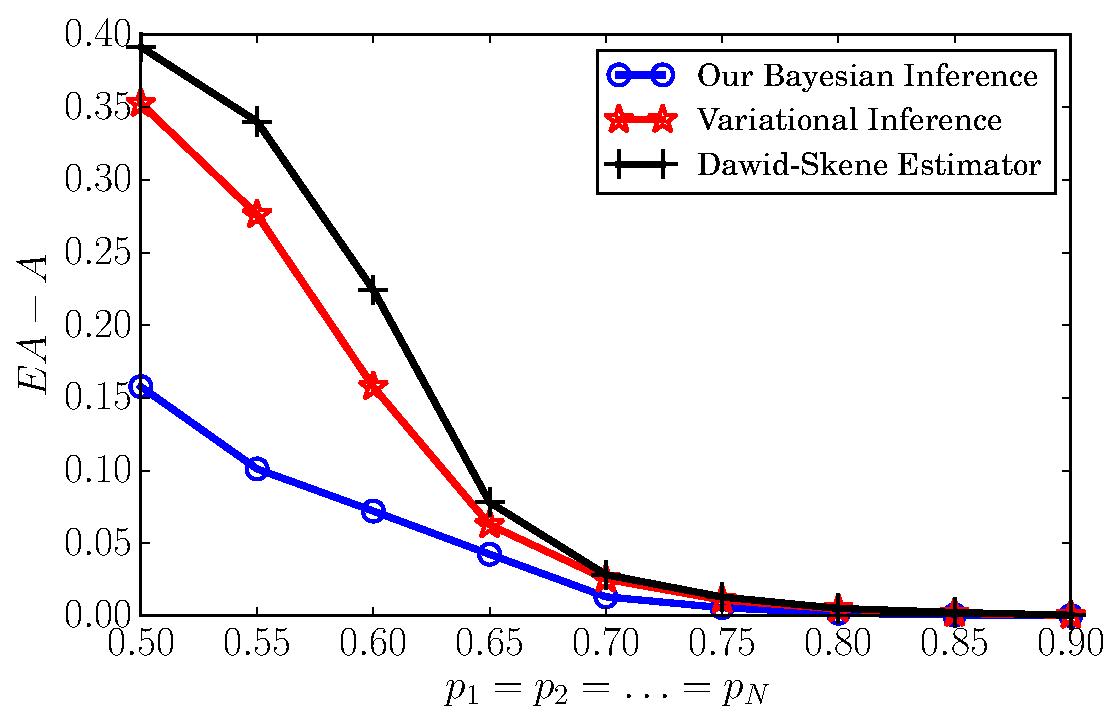
\includegraphics[width=\textwidth]{image/EXPC1}
        \caption{\label{BPP1}Changing the true label distribution}
    \end{subfigure}
    ~
    \begin{subfigure}[t]{0.24\textwidth}
        \centering
        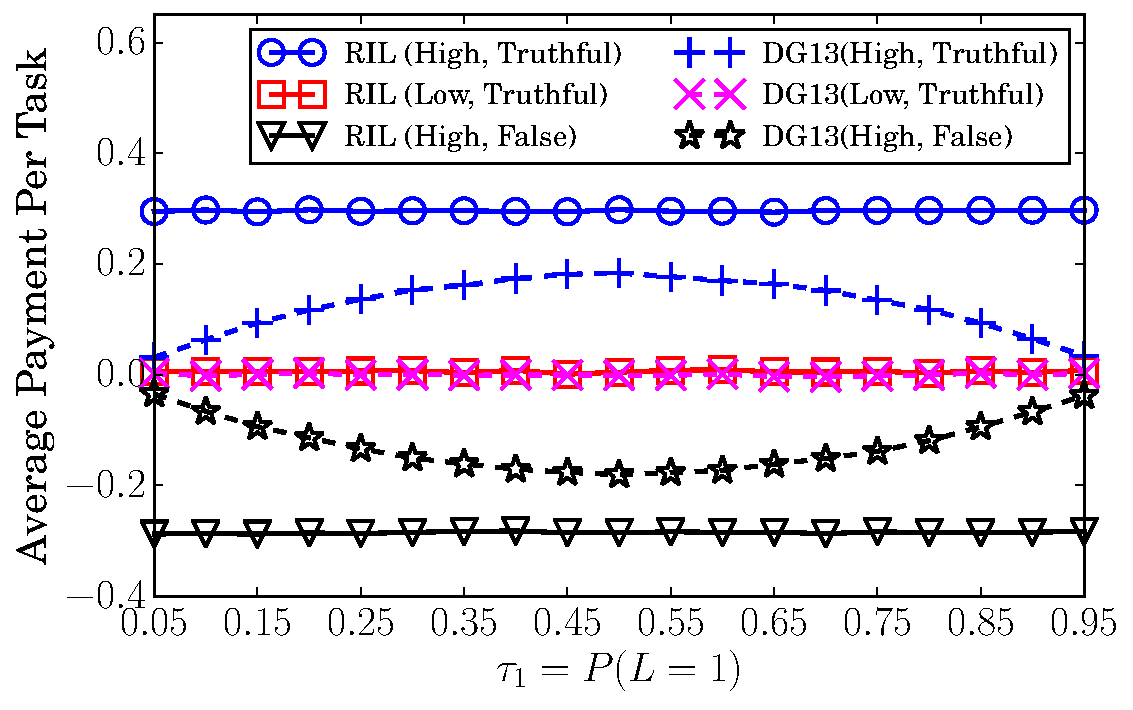
\includegraphics[width=\textwidth]{image/BPP1}
        \caption{\label{BPP1}Changing the true label distribution}
    \end{subfigure}%
    ~
    \begin{subfigure}[t]{0.24\textwidth}
        \centering
        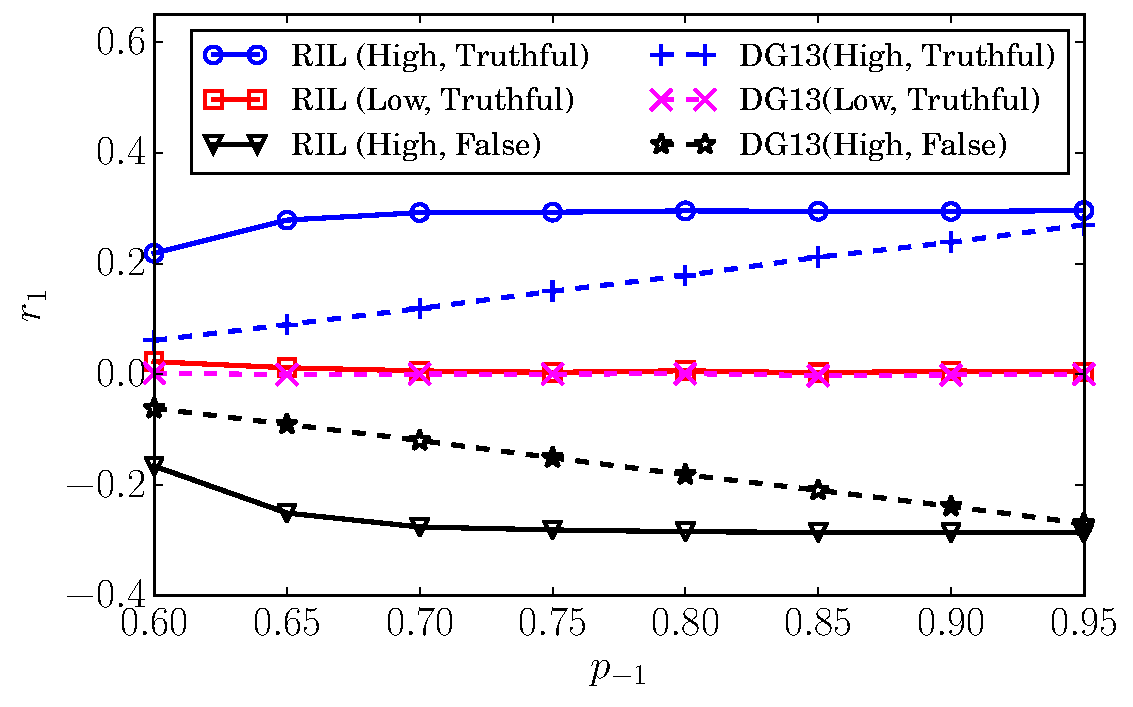
\includegraphics[width=\textwidth]{image/BPP2}
        \caption{\label{BPP2}Changing the opponent workers}
    \end{subfigure}
        ~
    \begin{subfigure}[t]{0.24\textwidth}
        \centering
        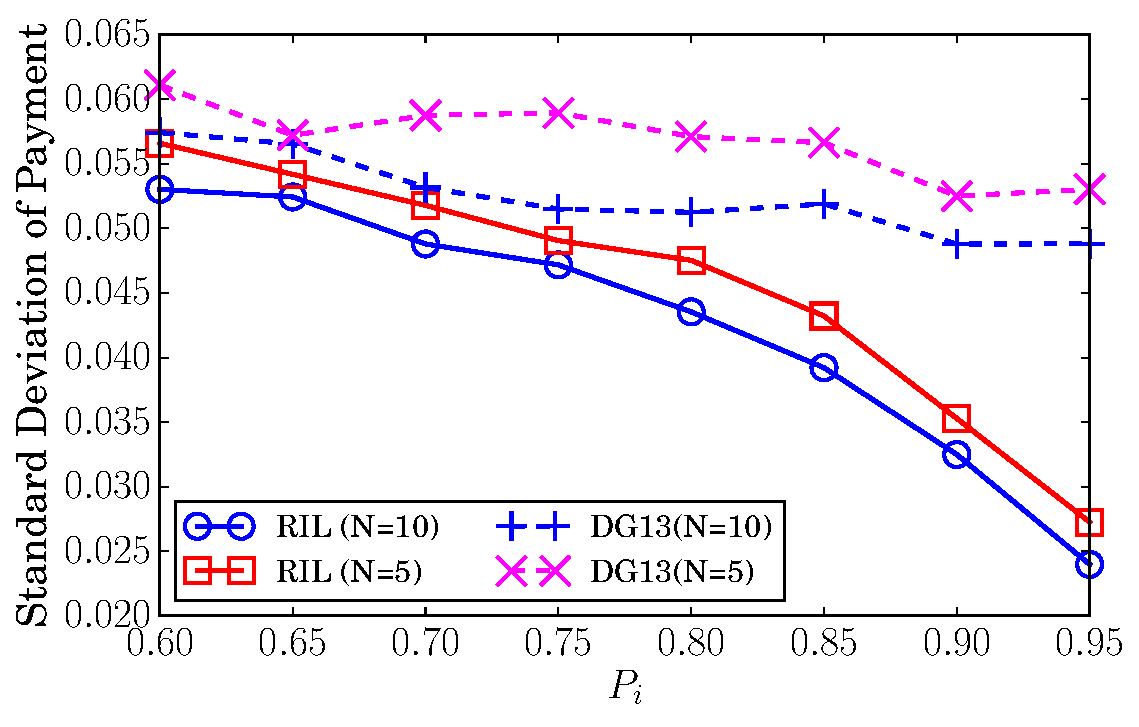
\includegraphics[width=\textwidth]{image/BPP3}
        \caption{\label{BPP3}Changing the targeted worker}
    \end{subfigure}
    \caption{\label{BPP}Empirical analysis on the incentive received by worker $1$}
\end{figure*}

%\begin{equation}
%P(L(j)=1)=\tau_1{\prod}_{k\neq i}p_H^{\delta_{kj1}}(1-p_H)^{\delta_{kj2}}
%\end{equation}
%where $\lambda_0=\log(\tau_1/\tau_2)$ and $\lambda_i=\log(p_i/\bar{p}_i)$. For worker $i$, we assume that all other workers report truthfully and exert high efforts. Suppose the real true label is $1$. In order to ensure $\mathbb{E}[m/M]$ to approach $0$, the probability ratio in Equation~\ref{Ratio} must be positive with almost $1.0$ probability. Thus, we can directly discard the absolute operation in Equation~\ref{vot} and calculate the expected value of task $j$ as
%\begin{equation}
%\mathbb{E}_1v(j)\approx \lambda_0+(N-1)(2p_H-1)\lambda_H+(2p_i-1)\lambda_i.
%\end{equation}
%Similarly, if the real true label is $2$, then
%\begin{equation}
%\mathbb{E}_2v(j)\approx -\lambda_0+(N-1)(2p_H-1)\lambda_H+(2p_i-1)\lambda_i.
%\end{equation}
%Thus, the average task value $v$ satisfies
%\begin{equation}
%\begin{split}
%&\mathbb{E}v = \tau_1 \mathbb{E}_1v(j) + \tau_2\mathbb{E}_2v(j)\\
%&=(2\tau_1-1)\lambda_0+(N-1)(2p_H-1)\lambda_H+(2p_i-1)\lambda_i.
%\end{split}
%\end{equation}
%
%Suppose the true label is $1$.
%\begin{equation}
%x= \log\frac{P(L=1)}{P(L=2)}=g+\sum_{i=1}^{N}f(x_i,y_i,w_i,z_i)
%\end{equation}
%\noindent where $g=g_1-g_2$, and 
%\begin{equation*}
%g_1=\log(s_1+t_2+1)\;,\;g_2=\log(s_2+t_1+1).
%\end{equation*}
%Omitting the subscript in $f$, we can have $f=f_1-f_2$ with probability $p$ and $f=f_2-f_1$ with probability $1-p$. Here,
%\begin{equation*}
%f_1=\log(x+z+2)\;,\;f_2=\log(w+y+1).
%\end{equation*}
%Thus, we can have
%\begin{equation}
%\mathbb{E}g = \mathbb{E}g_1-\mathbb{E}g_2 \;,\;
%\mathbb{E}f = (2p-1)(\mathbb{E}f_1-\mathbb{E}f_2).
%\end{equation}
%From the previous proof, we know that $P(m)$ is very small when $m>>1$. Thus, we mainly focus on the region where $m$ is relatively small. For a given small $m$,
%\begin{equation}
%\mathbb{E}_{s_1, t_2}g_1\approx \mathbb{E}_{t_2}\log(np+t_2+1)
%\end{equation}
%\begin{equation}
%\log(np+t_2+1) = \log(np+1)+\sum_{i=1}^{\infty}(-1)^{i-1}q^i
%\end{equation}
%\begin{equation}
%q = \frac{t_2}{np+1}\Rightarrow 0\leq q^{i} \leq c^{i}\cdot \left(\frac{m}{M}\right)^i\leq c^{i}\frac{m}{M}
%\end{equation}
%Then,
%\begin{equation}
%\mathbb{E}g_1 \approx \mathbb{E}_{m}\log(1+Mp-mp)
%\end{equation}
%\begin{equation}
%\log(1+Mp-mp)\approx\log(1+Mp)+\sum_{i=1}^{\infty}(-1)^{i}\left(\frac{m}{M}\right)^i
%\end{equation}
%Using the similar way of approximation for the computation of $\mathbb{E}g_2$, $\mathbb{E}f_1$ and $\mathbb{E}f_2$, we can have
%\begin{equation}
%\begin{split}
%\mathbb{E}g_1\approx \log(Mp)\;,\;\mathbb{E}g_2\approx \log(M(1-p))\\
%\mathbb{E}f_1\approx \log(Mp)\;,\;\mathbb{E}f_2\approx \log(M(1-p))
%\end{split}
%\end{equation}
%Thus, if all workers exert high efforts and report truthfully,
%\begin{equation}
%    \mathbb{E}x \approx \log\lambda_0 + {\sum}_{i=1}^{N}\log\lambda_{i,H}
%\end{equation}
%If the true label is $2$, then
%\begin{equation}
%    \mathbb{E}x \approx \log\lambda_0 - {\sum}_{i=1}^{N}\log\lambda_{i,H}
%\end{equation}
%Thereby,
%\begin{equation}
%    \mathbb{E}|x|\approx (2p_0-1)\log\lambda_0+ {\sum}_{i=1}^{N}\log\lambda_{i,H}
%\end{equation}
%When, for example, worker $1$ deviate from the desired equilibrium strategy, the non-equilibrium state correspond to
%\begin{equation}
%    \mathbb{E}|x'|\approx (2p_0-1)\log\lambda_0+ \log\lambda_{1}+{\sum}_{i=2}^{N}\log\lambda_{i,H}
%\end{equation}
%The minimal value of $\mathbb{E}|x'|$ is reached when worker $1$ exert high efforts and report falsely, namely $\log\lambda_{i}=-\log\lambda_{i,H}$.
%Thus, the maximal reward increment brought by worker $1$'s strategy switch is
%\begin{equation}
%    V_1 = F(\mathbb{E}x)-F(\mathbb{E}x') \approx 2\log\lambda_{1,H}\cdot \left.\frac{\mathrm{d}F}{\mathrm{d}x}\right|_{x=x_H}
%\end{equation}
%Since $p_0$ is difficult to estimate, we define the upper bound of the value increment as
%\begin{equation}
%    V = 2\max_{i}\log\lambda_{i,H} \cdot  \max_{x\in [x_H, \infty)}\frac{\mathrm{d}F}{\mathrm{d}x} 
%\end{equation}
%where $x_H= \log\lambda_0 + {\sum}_{i=1}^{N}\log\lambda_{i,H}$.
%Considering the discounted reward calculation in reinforcement learning, we can know the maximum value difference can be created by the manipulation of any worker is $(1-\rho)^{-1}V$. Meanwhile, if the reinforcement part increases the scaling factor by $\delta$ to obtain the reward increment, we need to pay more than $\sum_{i=1}^{N}M\delta (p_{i,H}-0.5)$. Thus, if we want to prevent the reinforcement learning module from the adversarial manipulation, the minimal gap $\delta$ between to two available scaling factors should satisfy
%\begin{equation}
%    \sum_{i=1}^{N}M\delta (p_{i,H}-0.5) > V.
%\end{equation}

\bibliographystyle{named}
\bibliography{ref}

\end{document}


% This document was modified from the file originally made available by
% Pat Langley and Andrea Danyluk for ICML-2K. This version was created
% by Iain Murray in 2018. It was modified from a version from Dan Roy in
% 2017, which was based on a version from Lise Getoor and Tobias
% Scheffer, which was slightly modified from the 2010 version by
% Thorsten Joachims & Johannes Fuernkranz, slightly modified from the
% 2009 version by Kiri Wagstaff and Sam Roweis's 2008 version, which is
% slightly modified from Prasad Tadepalli's 2007 version which is a
% lightly changed version of the previous year's version by Andrew
% Moore, which was in turn edited from those of Kristian Kersting and
% Codrina Lauth. Alex Smola contributed to the algorithmic style files.
